\chapter{Algebra Linear}

\section{Operações Vetoriais}
ADIÇÃO DE DOIS VETORES

PRODUTO POR UM ESCALAR

\subsection{Produto Escalar de dois vetores}

\begin{equation}\label{6.1}
    \textbf{A} \cdot \textbf{B} = AB \cos \theta
\end{equation}

COMUTATIVA

DISTRIBUTIVA
\begin{equation}\label{6.2}
    \textbf{A} \cdot (\textbf{B}+\textbf{C})=\textbf{A} \cdot \textbf{B}+\textbf{A} \cdot \textbf{C}
\end{equation}

PRODUTO VETORIAL DE DOIS VETORES

\section{Vetor na forma de componentes retângulares}

PRODUTO TRIPLO

\section{Giro dos Eixos Coordenados}\nocite{weber2003essential}

\begin{equation}\label{6.3}
\begin{split}
    (x,y)&=x(1,0)+y(0,1)\\
    &=x(\cos \phi , \sin \phi)+y(-\sin \phi , \cos \phi)\\
    &=(x\cos \phi - y\sin \phi, x \sin \phi +  \cos \phi )
    \end{split}
\end{equation}

As coordenadas do ponto $P(x,y)$ após girar $\phi$ graus envolta da origem terá (em relação ao plano). Ou seja, temos após o giro:
\begin{center}
 $P'= \begin{cases}
x'=x\cos \phi - y\sin \phi \\ 
y'= x \sin \phi +  y\cos \phi
\end{cases}$
\end{center}
Ou ainda

$$\left( \begin{matrix} x' \\ y' \end{matrix} \right)=\begin{bmatrix} \cos \phi & \sin \phi \\ -\sin \phi  & \cos \phi \end{bmatrix}\left( \begin{matrix} x \\ y \end{matrix} \right) $$

Quanto é o plano e não o ponto que gira entorno da origem então é como se o ponto girasse no sentido oposto do ponto de vista do plano. Ou seja, se o plano gira $\phi$ graus e o ponto \textit{P} permanece parado então é como se o plano tivesse se mantido parado e o ponto tivesse girado $-\phi$ graus, ou girado $\phi$ no sentido oposto. Logo teremos

\begin{equation}\label{6.4}
\begin{split}
    (x',y')&=x(\cos (-\phi) , \sin (-\phi))+y(-\sin (-\phi) , \cos (-\phi))\\
    &=x(\cos \phi , -\sin \phi)+y(\sin \phi , \cos \phi)\\
    &=(x\cos \phi + y\sin \phi,- x \sin \phi + y \cos \phi )
    \end{split}
\end{equation}

Ou seja:

\begin{center}
$ P'= \begin{cases}
x'=x\cos \phi + y\sin \phi \\ 
y'=- x \sin \phi + y \cos \phi
\end{cases}$
\end{center}

Podemos deduzir essa mesma fórmula apartir da imagem abaixo. Note que temos dois triângulos retângulos em que as hipotenusas são a coordenada e a abscissa.  Note ainda que o ângulo mais agudo de ambos corresponde a $\phi$. 

\begin{figure}[h]
    \centering
    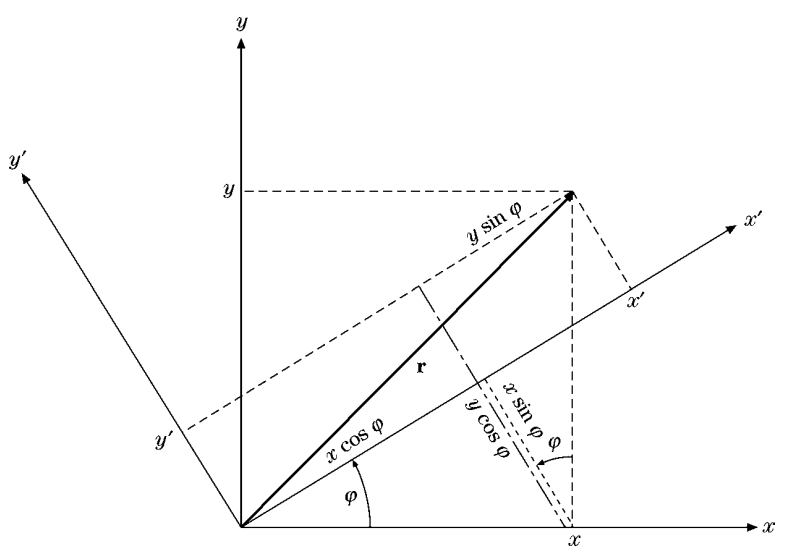
\includegraphics[scale=.5]{./imagens/09.png}
    \caption{Coordenadas de um ponto em um plano rotacionado}
    \label{fig:my_label}
\end{figure}


